\chapter{Scheduler Tool}
\label{chapter:scheduler}
The scheduler is a tool which accepts the information about the hardware configuration 
and matrix structure to generate a instruction stream and BRAM memory map
for all the elements of input matrix as well as the generated factors. For a 
given circuit this tool has to be used only once. After that generated information 
can be used for subsequent iterations. The operation of the scheduler tool is divided onto 
three major phases: 
\begin{enumerate}
    \item Input processing, Symbolic analysis and Memory Allocation
    \item Scheduling 
    \item Intersection stream and Memory map generation
\end{enumerate}

\section{Input Processing}
The scheduler tool accepts the input matrix data in the Compressed Column Sparse (CCS)
format. Also it requires the hardware configuration information as follows:
\begin{multicols}{2}
    \begin{itemize}
        \item Number of BRAM blocks
        \item Number of MAC units
        \item Number of divider units
        \item Latency of all the units
        \item Number of ports available at each BRAM
        \item Address depth of BRAMs
    \end{itemize}
\end{multicols}
The preprocessing process ensures that the  on-chip memory is sufficient to perform the 
operation.

\section{Symbolic Analysis}
The aim of symbolic analysis is to find the set of non-zero locations (\(\chi\)). 
This can be achieved using the second part of Gilbert-Peierls' algorithm (Algorithm \ref{algo:GP_tri}).
The non-zero elements in column $i$ can be found using the following equations:

\begin{subequations}
    \centering
    \begin{align}
        (b_i \neq 0) &\implies (x_i \neq 0) \\
        (x_j \neq 0) and \exists i(l_{ij} \neq 0) &\implies (x_i \neq 0)
    \end{align}
    \label{eqn:sym:findingX}
\end{subequations}

\begin{figure}[h]
    \centering
    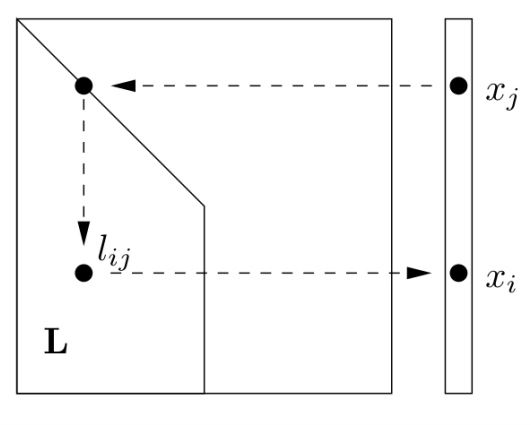
\includegraphics[width = 0.45\textwidth]{./Theory/nnzPattern.JPG}
    \caption{Non-zero pattern in LU decomposition}
    \label{fig:sym:nnzPattern}
\end{figure}

These two implications can be modelled as a traversal of a DAG representing the 
column dependance of the lower triangular section of graph $A$ \cite{Nechma}.
The set ($S$) of non-zero elements in any column ($j$) is given by 
\begin{equation}
    \centering
    s = \bigcup \limits_{x_{ij} \in a_j} Reach(x_{ij})
    \label{eqn:symNZ}
\end{equation}
where $a_j$ is a column vector of matrix $A$ and the $Reach(x)$ is defined as the 
location of non-zero elements in the $x^{th}$ column of the factor matrix which below the diagonal of the matrix. 
The reach of each column then has to be updated as fill ins may have been added to the column of factor matrix.
The location of fill-ins can be found
by removing the non-zero locations in $a_{ij}$ from $S$ as follows:
\begin{equation}
    \centering
    fillIn(j) = reach(j) - \{i|x_{ij}\neq 0\}
    \label{en:fillIns}
\end{equation}
To illustrate the algorithm consider the matrix $A$ shown in the following figure
\ref{fig:sym:example}. The bullets $(\bullet)$ represent non zero entries in the original matrix
and the circles $(\circ)$ represent the location of fill-ins. For example if we look 
at the column zero, it has non-zero elements at row indices 2 and 3. Therfore the $Reach(0) = \{2, 3\}$. It means that
any column with column index greater than 0 having a non-zero element at row index 0
will have non-zero elements at the row indices 2 and 3. Since columns 2 and 4 
satisfy the above condition they have non-zero elements at row indices 2 and 3 in the
factor matrix.

\begin{equation*}
    \begin{split}
        NonZero(Col_2) &= Reach(0, 2, 5) \\
        &= Reach(0) \cup Reach(2) \cup Reach(5) \\
        &= \{0, 2, 3\} \cup \{2, 5\} \cup \{5\} \\
        &= \{0, 2, 3, 5\}
    \end{split}
\end{equation*}

and hence the new reach of column 2 is $\{2, 3, 5\}$ location of fill-ins in column 2 are

\begin{equation*}
    \begin{split}
        fillIns(Col_2) &= Reach(2) - \{0, 2, 5\} \\
        &= \{3\}
    \end{split}
\end{equation*} 

\begin{figure}[h]
    \centering
    \begin{subfigure}[b]{0.5\textwidth}
        \centering
        \begin{tabular}{|c|c|c|c|c|}
        \hline
        \cellcolor{gray!80} $\bullet$   &                               &         $\bullet$            &                               &         $\bullet$     \\ 
        \hline
        \cellcolor{gray!80}             & \cellcolor{gray!80} $\bullet$ &                               &      $\bullet$                &                     \\ 
        \hline
        \cellcolor{gray!80} $\bullet$   & \cellcolor{gray!80}           & \cellcolor{gray!80} $\bullet$ &                               &          $\circ$    \\ 
        \hline
        \cellcolor{gray!80} $\bullet$   & \cellcolor{gray!80} $\bullet$ & \cellcolor{gray!80} $\circ$   & \cellcolor{gray!80} $\bullet$ &         $\circ$           \\ 
        \hline
        \cellcolor{gray!80}             & \cellcolor{gray!80}           & \cellcolor{gray!80} $\bullet$ & \cellcolor{gray!80}           & \cellcolor{gray!80} $\bullet$ \\ 
        \hline
        \end{tabular}
        \caption{Matrix with asymmetric non-zero pattern}
        \label{fig:sym:exampleMat}
    \end{subfigure}%
    \begin{subfigure}[b]{.5\textwidth}
        \centering
        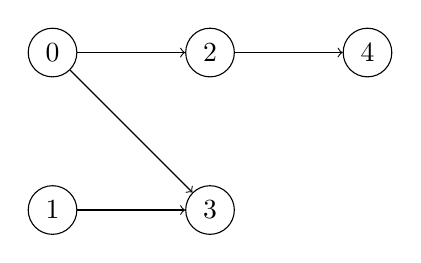
\begin{tikzpicture}
            \node[shape=circle,draw=black] (0) at (0,0) {0};
            \node[shape=circle,draw=black] (1) at (0,-2) {1};
            \node[shape=circle,draw=black] (2) at (2,0) {2};
            \node[shape=circle,draw=black] (3) at (2,-2) {3};
            \node[shape=circle,draw=black] (4) at (4,0) {4};

            \path [->] (0) edge (2);
            \path [->] (2) edge (4);
            \path [->] (0) edge (3);
            \path [->] (1) edge (3);
        \end{tikzpicture}
        \caption{Column dependency graph}
        \label{fig:sym:colDepGraph}
    \end{subfigure}
    \caption{Example of Symbolic Analysis}
    \label{fig:sym:example}
\end{figure}

\section{Generating Computational Flow Graph}

The computational flow graph is a directed acyclic graph of all the operations
which are required to compute the factor matrix. Each node of the graph represents
single arithmetic operation such as MAC and divide. The children nodes of a particular
node represents the elements required to compute the give node and hence the children
must be executed before executing the parent node. A calculation of single element
may require multiple MAC operations and may or may not require divide operation (normalization) depending
on the location of the element in the matrix. For example in the factorization of the example matrix 
(figure \ref{fig:sym:exampleMat})
$U_{3,4} = A_{3,4} - U_{2,4}L_{3,0} - U_{0,4}L_{3_2}$. Since there are multiple 
atomic MAC operations and we can not execute them parallelly, the scheduling has to schedule one ofter the another.
The scheduler can not determine which of the required multiplicands will be ready first using the flow graph.
The task graph must represent all the possibilities for the execution of particular node (figure \ref{fig:sym:example:mac}). This
problem is solved by generating super node for all the AMC operations required for particular element. 
which require more than one. This allows scheduler to determine the operation sequence 
based on the availability for operands.

\begin{figure}
    \centering
    \begin{subfigure}[t]{0.32\textwidth}
        \centering
        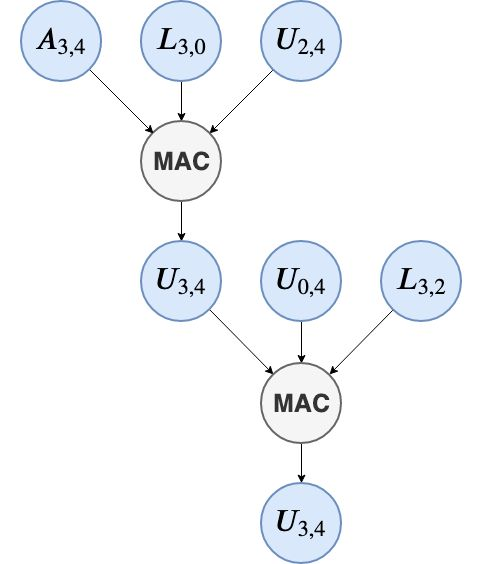
\includegraphics[width = \textwidth]{./Scheduler/macNode1.jpg}
        \caption{Dependency graph for the node $U_{3,4}$}
        \label{fig:sym:example:mac0}
    \end{subfigure}
    \hfill
    \begin{subfigure}[t]{0.32\textwidth}
        \centering
        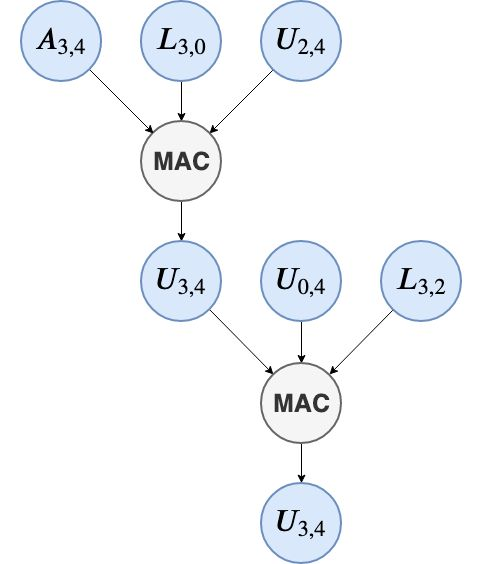
\includegraphics[width = \textwidth]{./Scheduler/macNode1.jpg}
        \caption{Execution option 1}
        \label{fig:sym:example:mac1}
    \end{subfigure}
    \hfill
    \begin{subfigure}[t]{0.32\textwidth}
        \centering
        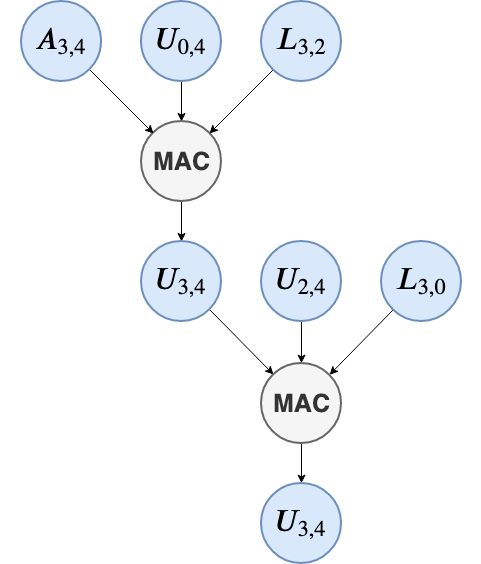
\includegraphics[width = \textwidth]{./Scheduler/macNode2.jpg}
        \caption{Execution option 2}
        \label{fig:sym:example:mac2}
    \end{subfigure}
    \caption{Example showing multiple possible computation flows for the single MAC element}
    \label{fig:sym:example:mac}
\end{figure}


The computation flow can be generated in symbolic analysis itself without much overload as we already know 
the positions of non-zero elements and the elements which are responsible for making them non-zero . 
The figure \ref{fig:sym:flowGraph} shows the 
computational flow graph for the example matrix shown in figure \ref{fig:sym:exampleMat}.

\begin{figure}
    \centering
    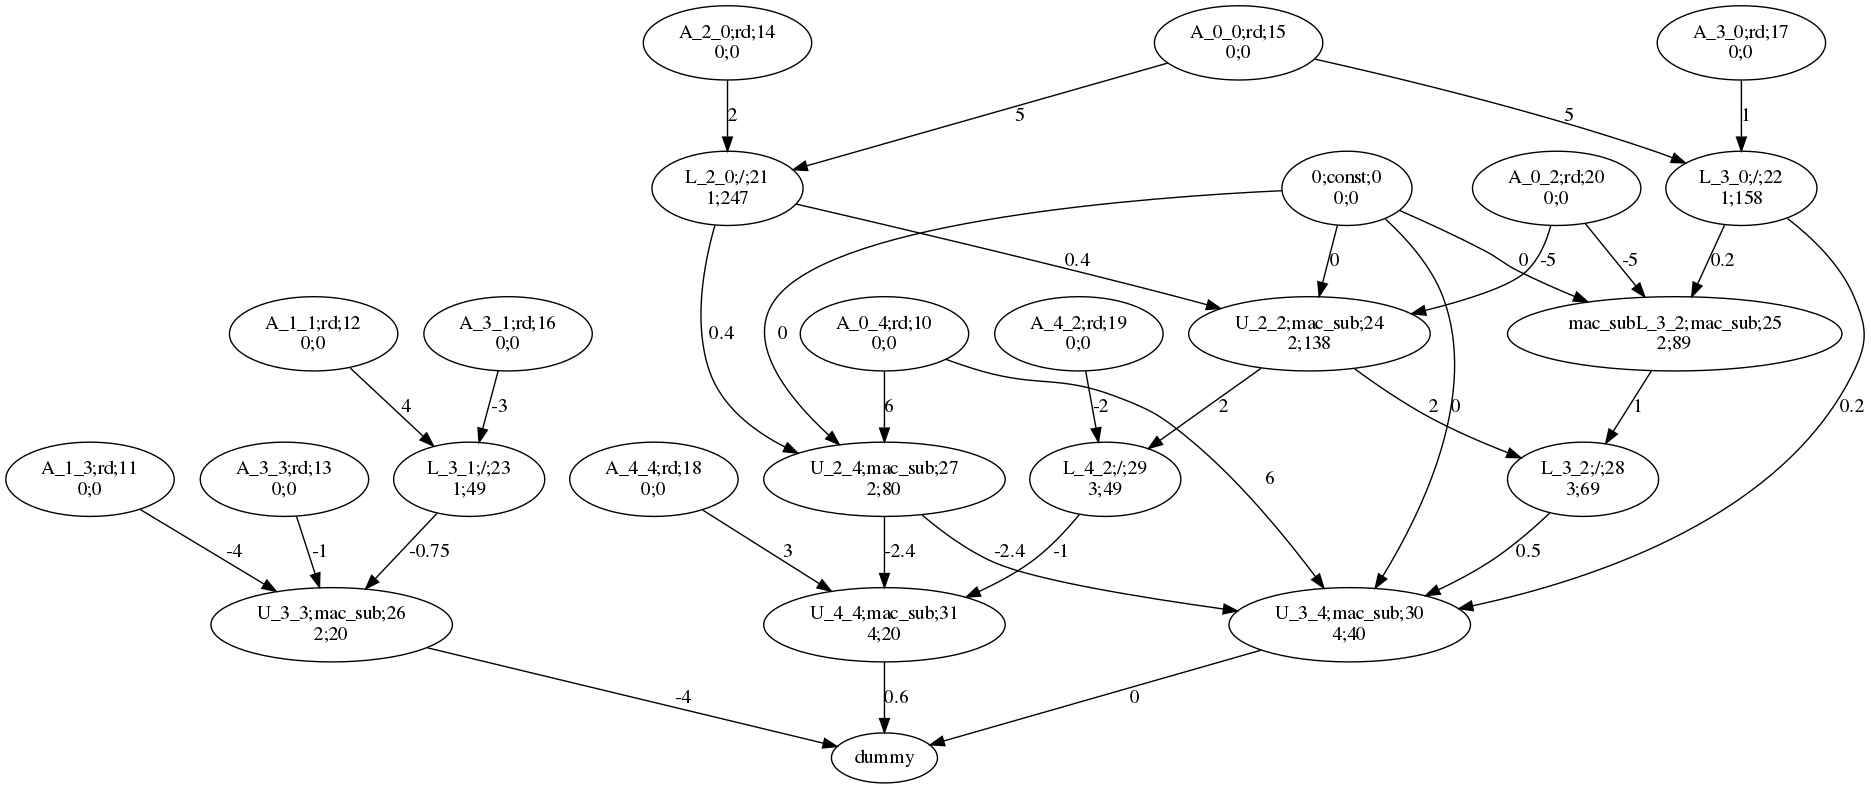
\includegraphics[width = \textwidth]{./Scheduler/exeTree.png}
    \caption{Computational flow graph for example matrix shown in figure \ref{fig:sym:exampleMat}}
    \label{fig:sym:flowGraph}
\end{figure}



\section{Memory Address Assignment}
Symbolic analysis determines location of all the non-zero elements in the factor matrix hence 
the amount of storage required to store both L and U matrices can be calculated. 
All the diagonal elements of the L factor matrix are zero and hence do not 
require memory storage an can be omitted from the process. Also the elements
of the original matrix ($A$) are used only once and occupy the memory space 
corresponding non-zero locations in the factor matrix. There are many ways to allocate memory addresses
to matrices. Following are the three simple ways to allocate address locations:
\begin{description}
    \item[Linear Address Allocation]: All the elements in the matrix are arranged linearly one after the other. This type of Allocation 
        reduces the data gathering overhead after the execution has finished but hinders the performance as most of the times all the elements 
        in one column are allocated in the same BRAM and cause read congestions.
    \item[Circular Address Allocation]: In this allocation policy the elements from the same column are circularly distributed 
        across all the BRAMs. 
\end{description}

\section{Scheduling}

The scheduling algorithm has to generate an execution schedule considering 
the hardware constraints and data dependencies. Since the hardware does not have
any dynamic problem handling capabilities the schedule generated must be 
cycle accurate and static. The scheduler uses ASAP strategy to assign the execution nodes.
A priority list is used to select the nodes from the pool of ready nodes. The priority
of the nodes is defined as:

\begin{equation}
    \centering
    Priority(n) = \sum_{i \in Parents(n)} Priority(i) + \sum_{x \in tasks(n)} Delay(x)
\end{equation}

where $Parents(n)$ is the set of nodes which are dependent on the node $n$ and $tasks(n)$ is the 
set of operations required to evaluate the node $n$. This definition of the priority 
ensures that the node which has more number of overall dependent nodes will be prioritized
by the greedy scheduling algorithm.
The important steps in the algorithm are as follows:

\begin{algorithm}
    \caption{Priority List based Scheduling Process}
        \label{algo:sch:sch}
    \begin{algorithmic}[1]
        \Require{$G$, a computation flow graph for LU decomposition}
        \Statex
        \State $scheduledNodes := 0$
        \State $readyNodes := G.leaves()$
        \While{$scheduledNodes < G.size()$}
            \State Update status of nodes retired in previous cycle
            \State Update scheduledNodes
            \State Update the ready nodes list
            \State Assign memory port to retiring nodes
            \State Calculate the free BRAM ports for reading and writing
            \State Select the most prior set of ready nodes which can be schedules in current cycle
            \State Assign the memory memory operations
        \EndWhile
    \end{algorithmic}
\end{algorithm}

\subsection{Finding Schedulable nodes}
The scheduler maintains two boolean state variables corresponding namely, $Dirty$ and $Done$ for each of the nodes. 
The set states of these variables indicate the following:
\begin{description}
    \item[$Dirty$]: The memory data corresponding to the node is outdated and must not be read
    \item[$Done$]: All the computations corresponding to node are done
\end{description}
The set state of $Done$ variable does not indicate that the data in the memory is accurate. $Dirty$ variable must be 
checked before accessing the data. These state variables ensure that the data being read always correct and also 
helps scheduler to properly manage the dependencies. At the start of each cycle, the scheduler 
has to find the set of ready nodes which can potentially form the execution assignment set for the cycle. such nodes 
are called as ready nodes.\\
The node is called ready when:
\begin{description}
    \item[MAC Node]: (Augend is not dirty or live) and at least one of addend pair of multiplicands is in done state.
    \item[Divide Node]: Both the operands must be in the done state. 
\end{description}
Since the ready state of nodes depends on the state of children nodes. This list is updates using the set 
of retiring nodes as they are fewer in number and anyway have to visited to generate write commands. \\

The schedular also maintains a list called as \textbf{Live Variables}, which represents the set of 
nodes whose correct values are available on the output ports of the PEs or BRAMs and hence can be 
read in current cycle. \\

Not all the nodes in the ready nodes are schedulable in current cycle. Some of operands 
corresponding the ready nodes may be dirty and hence have to removed from the 
schedulable node list. The list of live variables and the dirty state of operands is checked to
ensure the schedulability of individual the nodes. 


\subsection{Scheduling Table}
The scheduling algorithm uses a set of three tables (figure \ref{fig:sch:tableBlank}), assignment table, retirement table and 
memory operation table to keep track of all the assigned operation and determine the next set 
assignments. The schedular generates cycle accurate simulation and stores the assignments as
a set of instructions for the hardware. The top row of each table represents the current assignments
for each port. The tables are used to determine the future assignments. \\

\begin{figure}
    \centering
    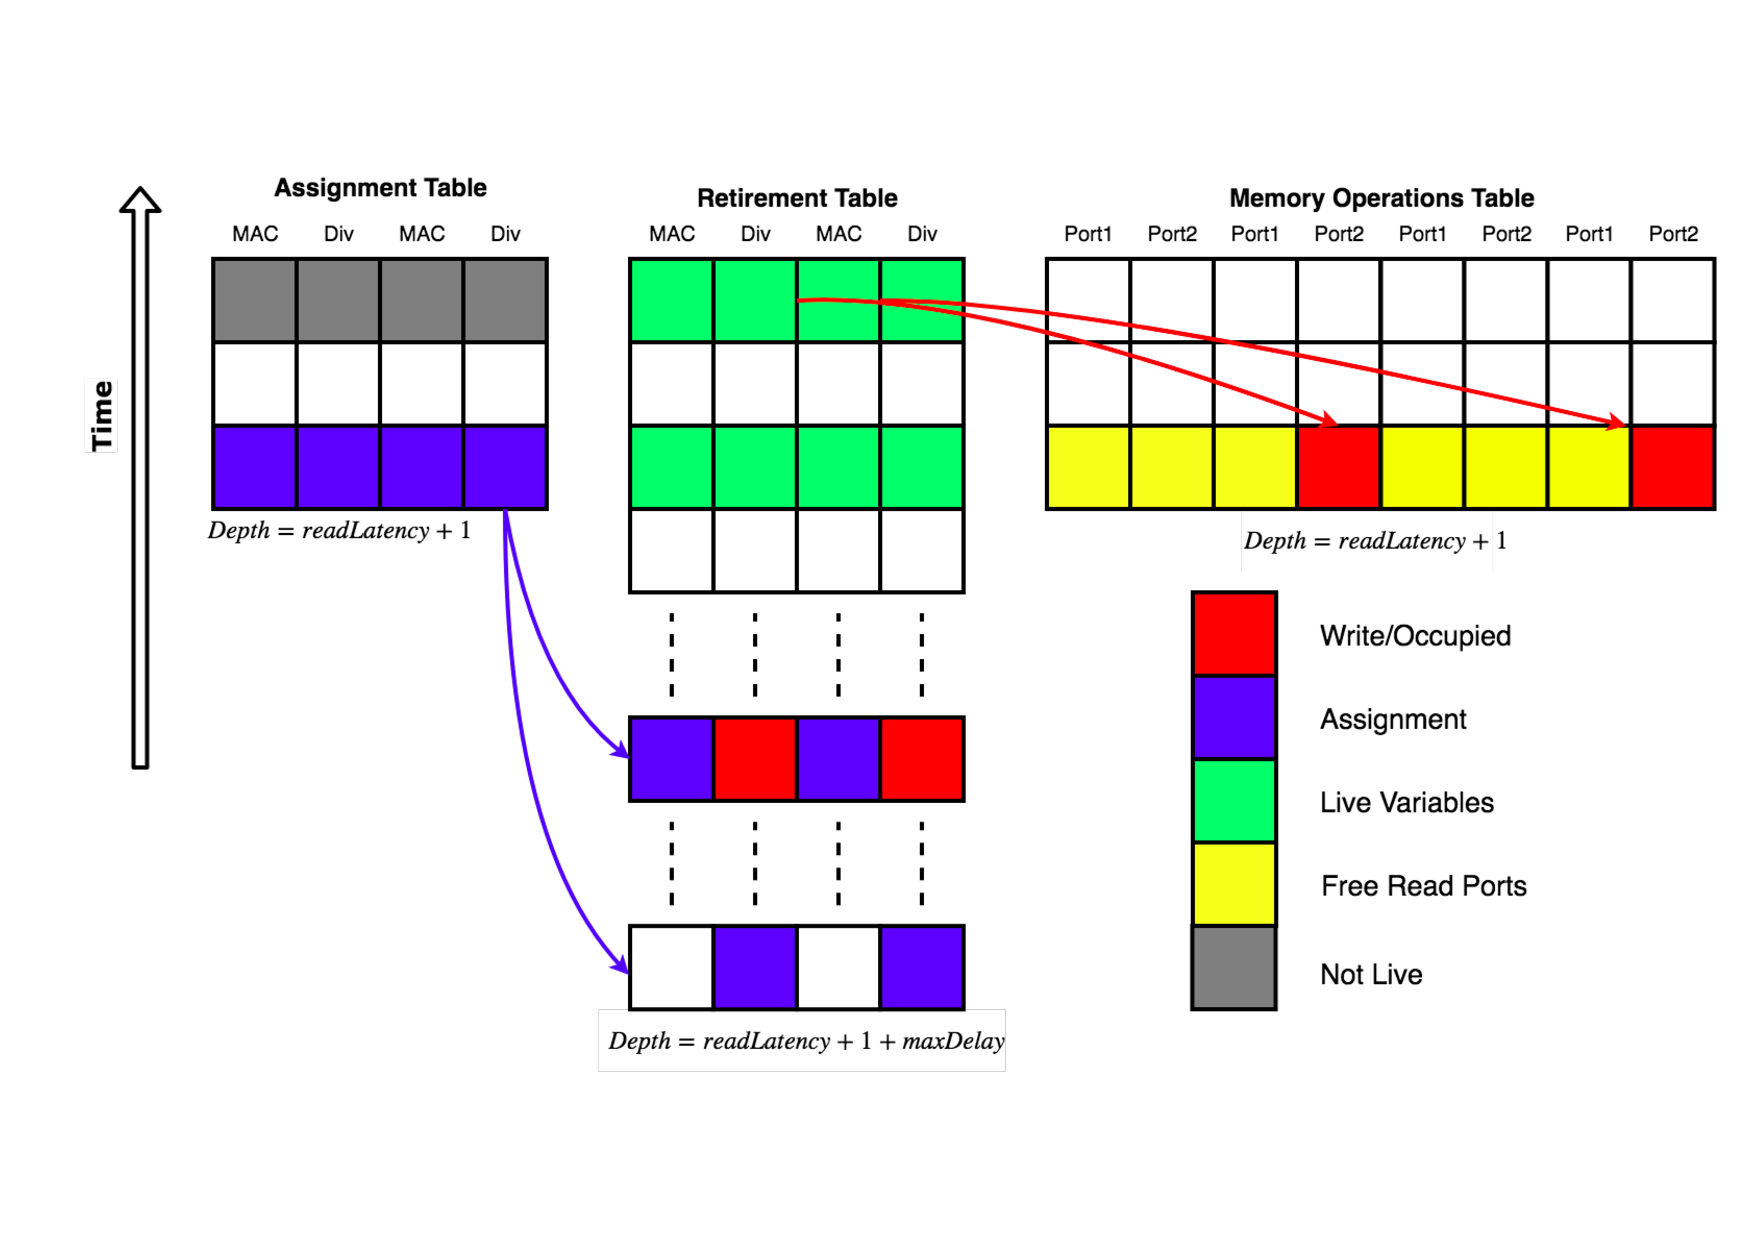
\includegraphics[width = \linewidth]{./Scheduler/schedulartable.pdf}
    \caption{Resource allocation tables used by schedular}
    \label{fig:sch:tableBlank}
\end{figure}

\textbf{Assignment Table}: \\
The top row of the assignment table represents the operations to be assigned at current cycle.
All the operation scheduled in a cycle must stored in the same cycle they retire because of unavailability 
of the output buffer. So the duplicate entries of the assigned operations are maid in the corresponding
retirement table cell. The top row of the table can be used to eliminate unnecessary writing of intermediate
results. \\

\textbf{Retirement Table}: \\
The top row of the retirement represents the operations retiring in the current cycle i.e. operations
whose results are available on the ooutput ports of PEs. These results must be written to the memory except in the case of 
write cancellation. \\
\pagebreak

\textbf{Memory Operation Table} \\
Memory operation table maintains the record of available ports and assigned operations. 
Operations are assigned to particular BRAM from the 0th port (time multiplexed ports 
are numbered from $0-(n-1)$) first order. The top row of the table indicates the memory 
operations in the current cycle.\\

\textbf{Selecting the set of assignments} \\
All the schedulable nodes are stored in the priority list in decreasing order. All combinations of nodes are 
checked for availability of BRAM ports for both reading and retirement. A valid combination with
highest sum of priorities is selected as assignments for the current cycle. Since this is the most
complex process (in therms of time complexity) and is in the critical path of the algorithm the size 
of the priority list is restricted to 100. 




\subsection{An Example of Scheduling Process}
Lets say at some clock cycle the nodes $n1_0$, $n2_0$, $n3_d$ are retiring 
and the nodes $n2_1$, $n4_d$, $n5_d$ are being assigned to the PEs. The BRAMs have read latency of two.
The schedulable list of nodes in the second next cycle can be calculated based on the current retiring nodes
and contains nodes $n6_2$, $n7_d$, $n8_d$, $n9_0$, $n10_0$

\begin{figure}
    \centering
    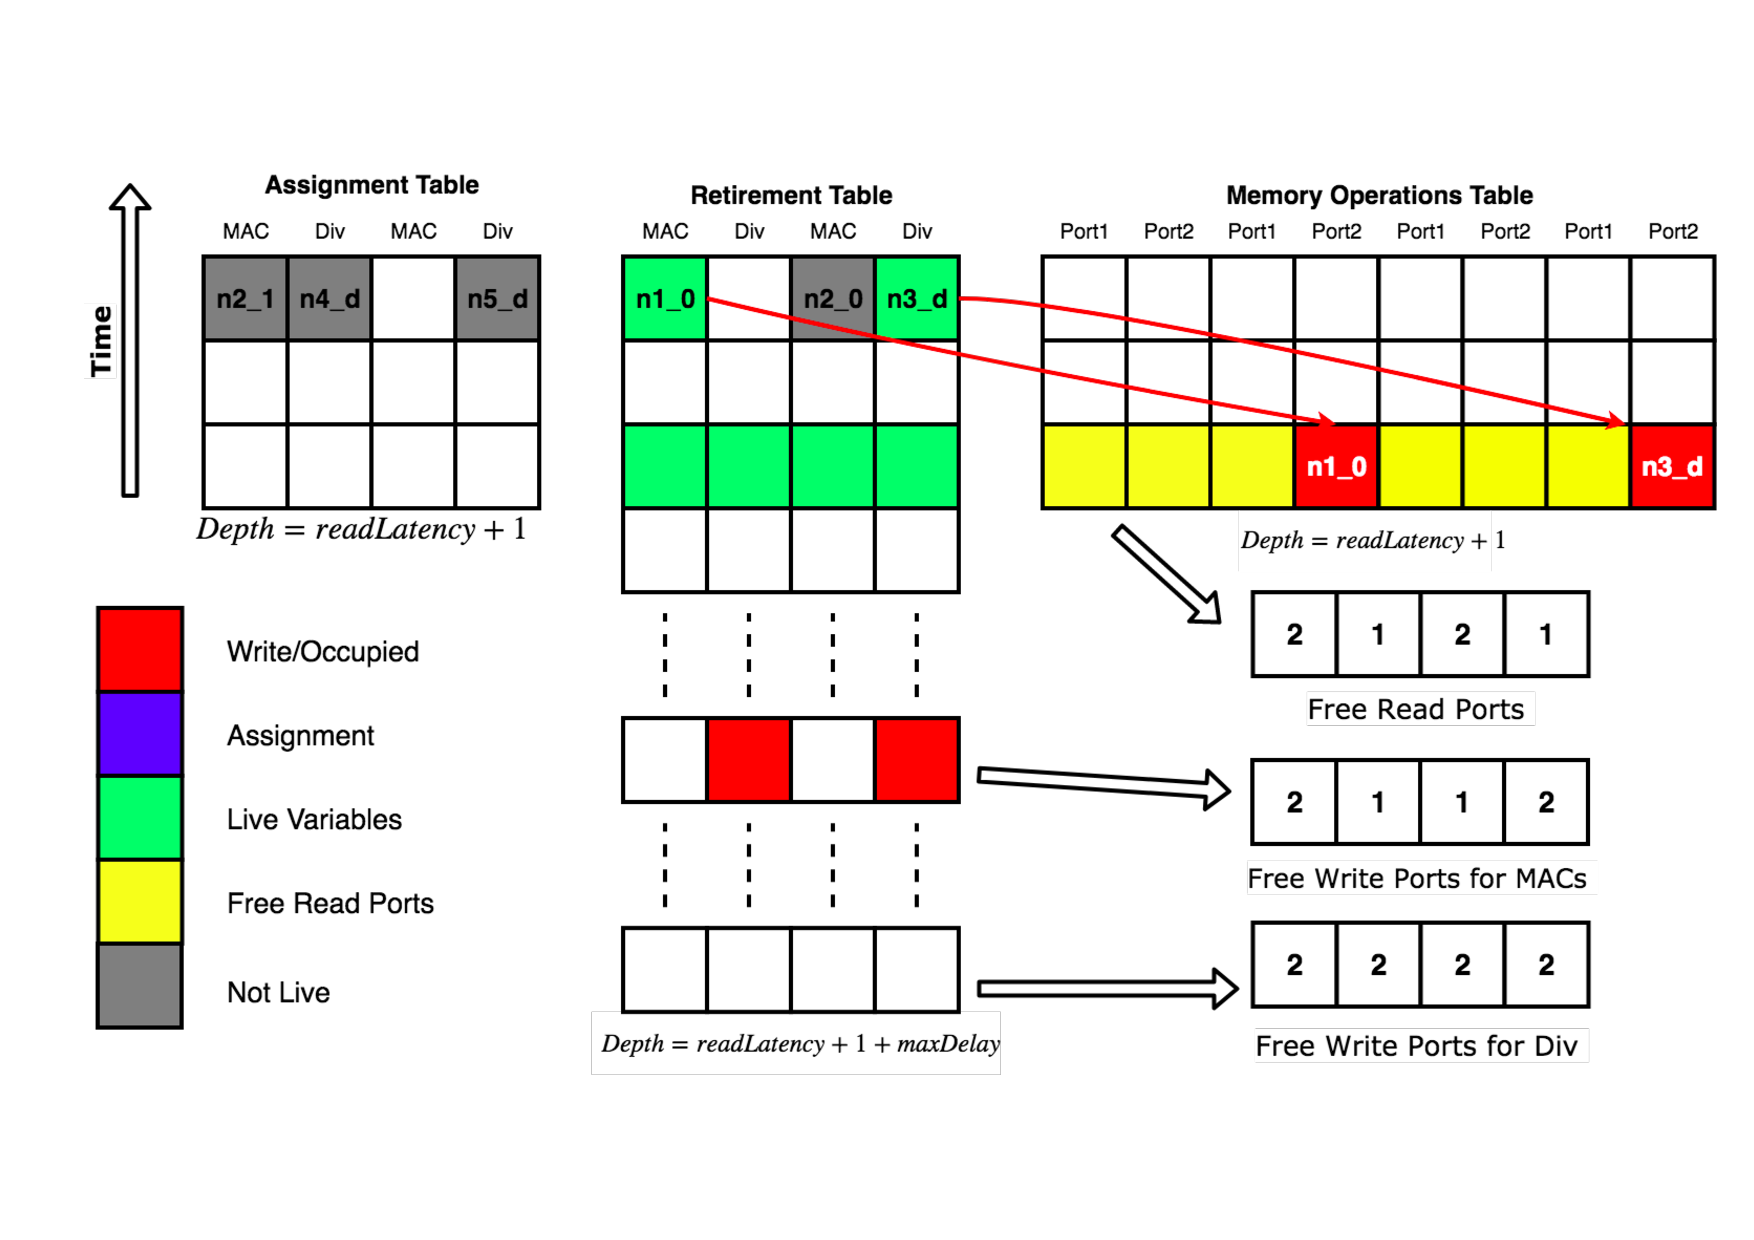
\includegraphics[width = \linewidth]{./Scheduler/exampleWrite.pdf}
    \caption{Selecting write ports}
    \label{fig:sch:exampleWrite}
\end{figure}

\textbf{Assigning Write Ports} \\
(Refer figure \ref{fig:sch:exampleWrite})
\begin{enumerate}
    \item Retiring nodes: $n1_0$, $n2_0$, $n3_d$
    \item Scheduled nodes: $n2_1$, $n4_d$, $n5_d$
    \item Scheduled node $n2_1$ utilizes the intermediate result generated from operation $n2_0$, hence the 
        write operation correspond to $n2_0$ can be eliminated. Hence the schedular has to reserve 
        only two write operations for remaining nodes $n1_0$ and $n3_d$.
    \item Now we can calculate free BRAM ports for read operations.
    \item Also we know the delay of each operation and hence determine calculate free PEs
        to assign operations.
\end{enumerate}

\begin{figure}
    \centering
    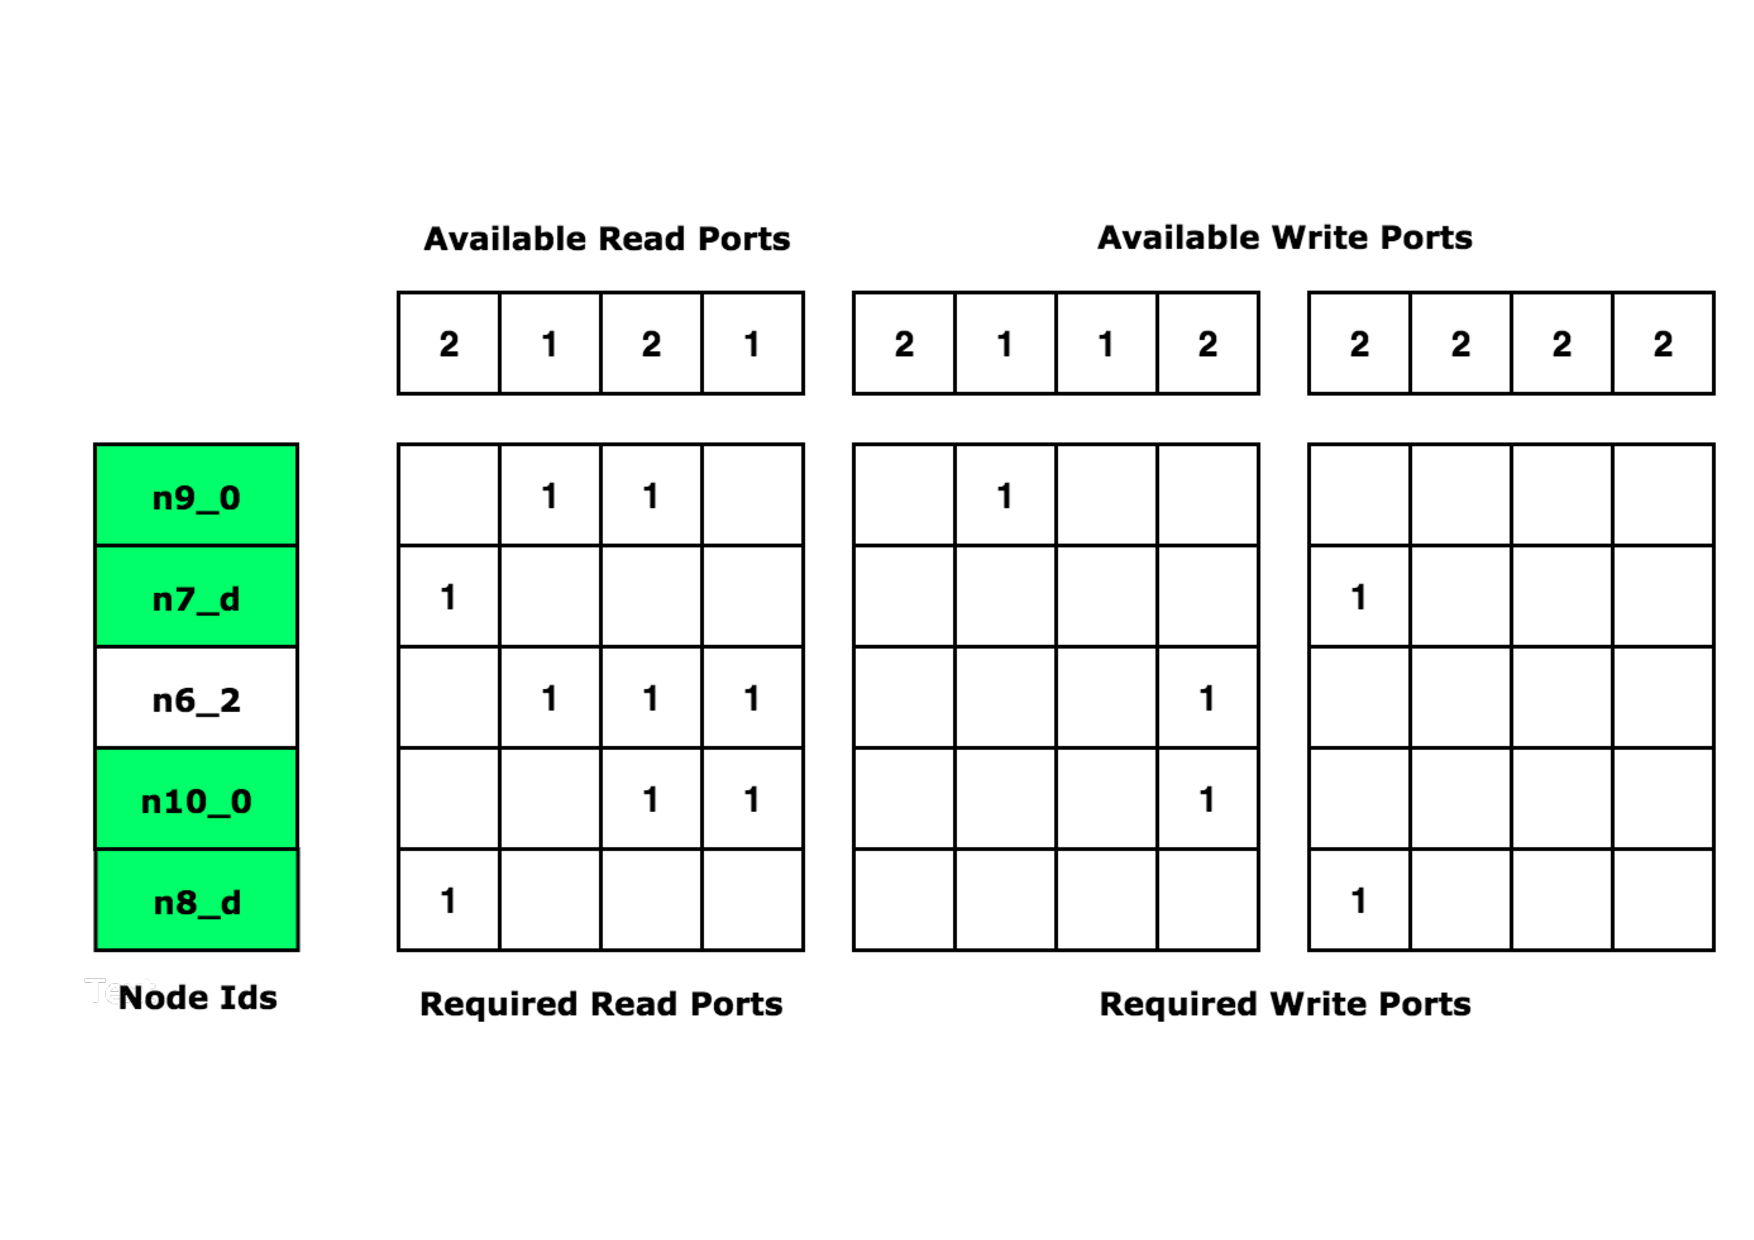
\includegraphics[width = 0.8\linewidth]{./Scheduler/examplePortSelection.pdf}
    \caption{Selecting operations}
    \label{fig:sch:exampleSelectPorts}
\end{figure}

\textbf{Operation Selection} \\
The figure \ref{fig:sch:exampleSelectPorts} shows 5 ready nodes and available ports.
The required number of read and write ports corresponding to each node for each BRAM are listed 
in the adjoining tables. A valid group of operations must have sum of ports required by selected nodes
should be less than total available nodes. The set with maximum sum of priorities
is assigned to to PEs in current scheduling cycle. In this case $n7_d$, $n8_d$, $n9_0$ and $n10_0$
forms the valid group and hence will be assigned at the bottom of the assignment table confirming the assignment in 
the second next clock cycle.
\\



\textbf{Memory Read Assignment}\\
One the assignments for the second next clock cycle ae decided, the additional 
required data values are set to be read from the corresponding memory locations in the
bottom row of the read allocation table.

\begin{figure}
    \centering
    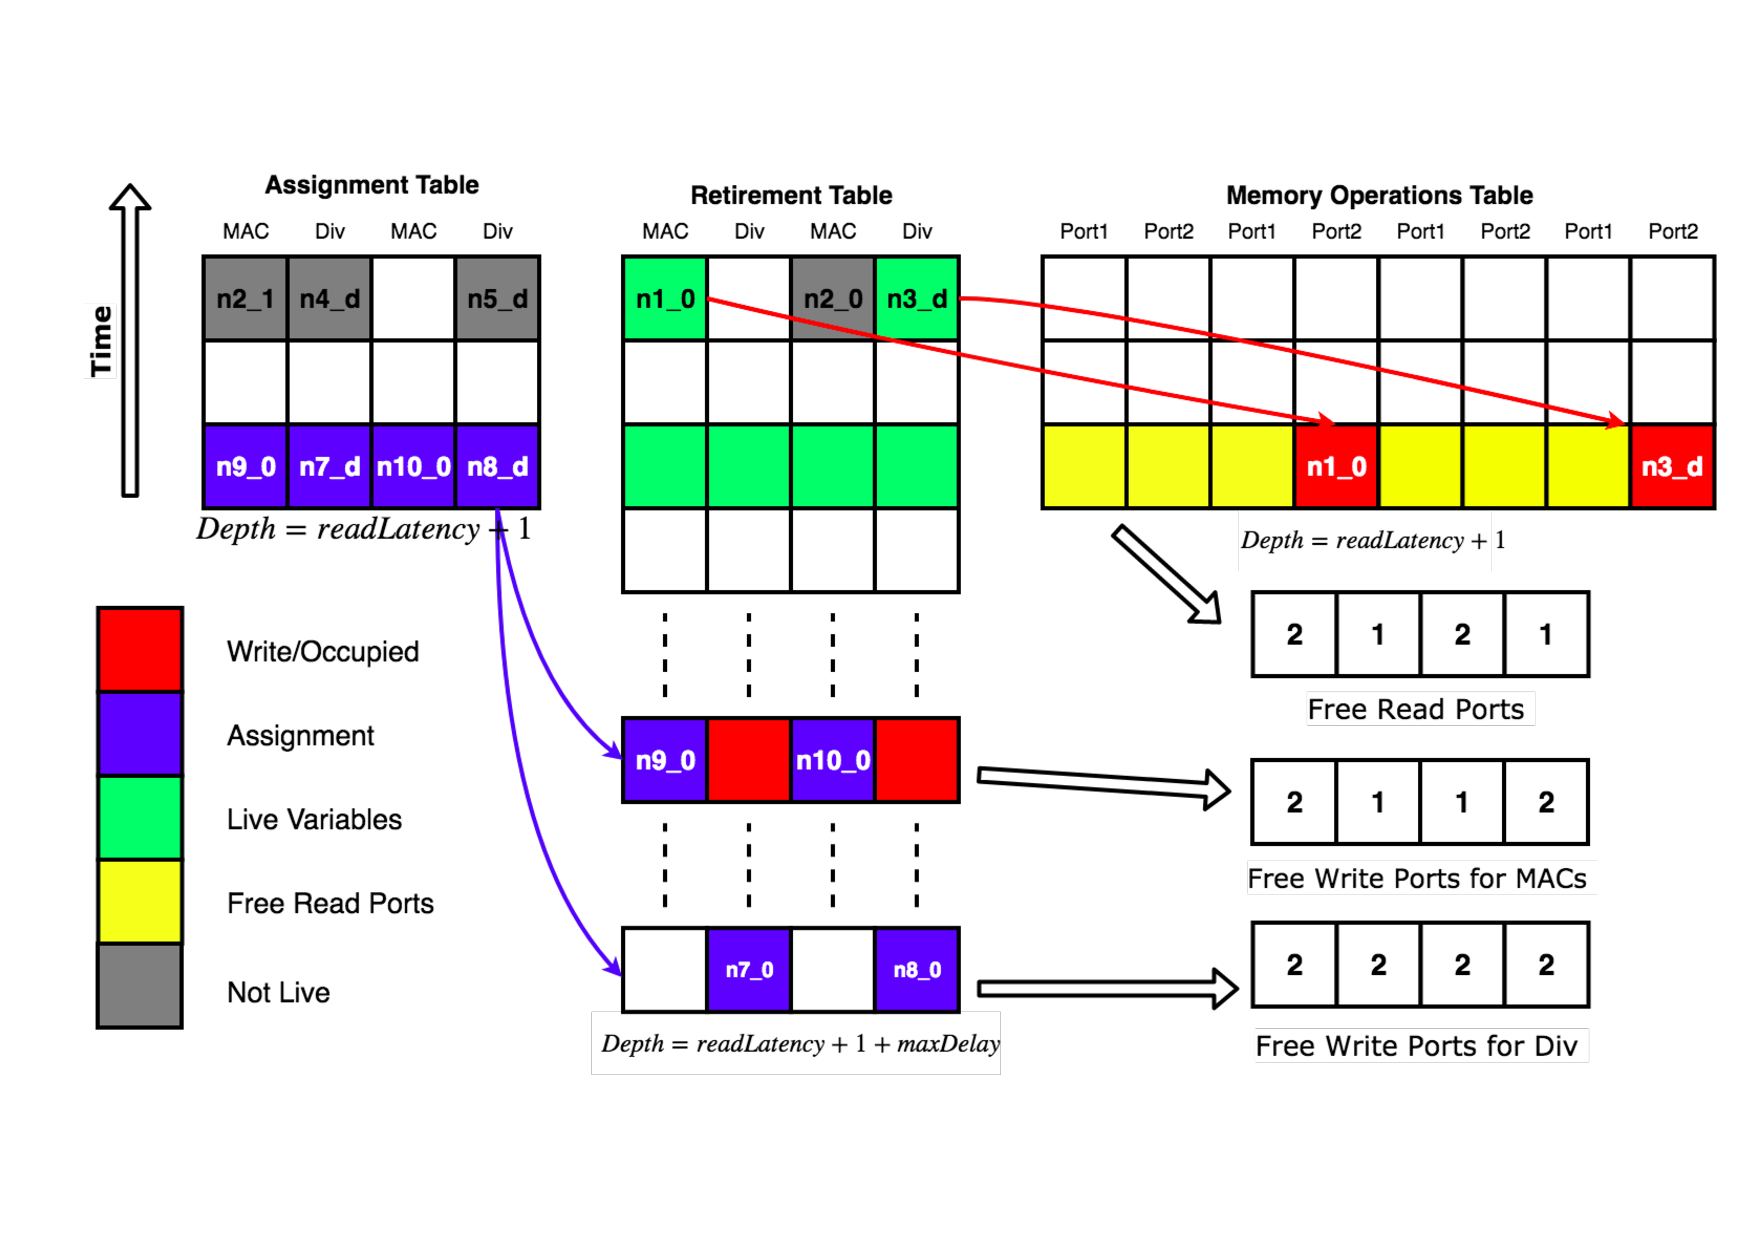
\includegraphics[width = \linewidth]{./Scheduler/exampleFinal.pdf}
    \caption{Final allocation}
    \label{fig:sch:exampleFinal}
\end{figure}

\textbf{Saving the Schedule} \\
Figure \ref{fig:sch:exampleFinal} shows the final allocation of the resources. 
All the non-zero allocations in the top row of each table are 
saved in the schedule vector. The table entries are then cleared. 
The tables ae stored as the two dimensional vector of structures. To avoid the huge amount
of memory relocation due to addition and deletion of new entries, the table indices
are accessed in rolling fashion i.e. the actual vector index for table at particular
cloak cycle is given by
$$
Vector\ Index  = (Table\ Index + Clock\ Cycle) \% Depth\ of\ Table
$$

% The scheduling algorithm uses the computational flow graph generated by symbolic 
% analysis step to schedule the operations while taking care of the conflicts.